\documentclass{IEEEtran}
\usepackage[utf8]{inputenc}
%\usepackage{fullpage}

\usepackage{amsmath}
\usepackage{graphicx}
\usepackage[colorinlistoftodos]{todonotes}
\usepackage[colorlinks=true, allcolors=blue]{hyperref}
\usepackage{mathtools}
\usepackage{latexsym}

\title{MeasureMesh: An Open Source Hardware/Software Platform for Flexible Data Logging}
\author{Matt Ruffner}
\date{}
\begin{document}

\maketitle

%%%%%%%%% ABSTRACT
% \begin{abstract}
% hello
% \end{abstract}



%%%%%%%%%%%%%%%%%%%%%%%%%%%%%
%%%%%%%%%%%%%%%%%%%%%%%%%%%%%
%%%%%%%%%%%%%%%%%%%%%%%%%%%%%
%%%%%%%%%%%%%%%%%%%%%%%%%%%%%
\section{Introduction}
 The Lora Alliance is a not profit association promoting the adoption of a Low Power Wide Area Network (LPWAN) IoT standard knows as Long Range WAN (LoRaWAN). It is a viable platform for low bandwidth, low power remote sensing applications. Over 100 complying companies adopt hardware standards including adaptive bitrate and encryption schemes specific to the LoRaWAN protocol.
 
LoRaWAN is commonly utilized for remote sensing applications including environmental and livestock monitoring~\cite{WuFan2018WAwI,IkhsanMukhammadGufron2018MLGf}. The LoRa standard is designed to be a low power solution, with longer range than traditional wireless means of communication (WiFi, Bluetooth, Zigbee, Z-Wave, etc.). It follows that compared to other wireless protocols, LoRa has significantly lower bandwidth and throughput~\cite{WuFan2018WAwI}. Performance measurements of certain LoRa chipsets have concluded that longer ranges are achievable in a rural setting with the lowest data rates, and that range in urban settings is less, requiring lower data rates at shorter distances than in rural settings~\cite{RamonSanchez-Iborra2018PEoL}. This suggests that dynamic tuning of the radio parameters is necessary based on deployment location. 

MeasureMesh builds on this LPWAN technology to providing a simple, adaptable hardware and software platform that facilitates easy adoption for custom remote sensing networks. By using off the shelf radios and control units for node and gateway hardware, quick time-to-implementation is achieved, allowing for more focus and customization on sensing needs. The gateway utilizes internet protocol for communicating with a server back-end. For the purposes of this paper, a simple sensor data storage back-end and plotting front-end will be implemented.
%%%%%%%%%%%%%%%%%%%%%%%%%%%%%
%%%%%%%%%%%%%%%%%%%%%%%%%%%%%
%%%%%%%%%%%%%%%%%%%%%%%%%%%%%
%%%%%%%%%%%%%%%%%%%%%%%%%%%%%
\section{Project Overview} 

MeasureMesh consists of a varying number of nodes which communicate to a gateway via LoRa packet radios. The gateway then logs collected data to a cloud databse via internet. Figure \ref{fig:mmoverview} shows the MeasureMesh Implementation of a typical LoRa network topology\footnote{https://lora-alliance.org/about-lorawan}, along with chosen implementation hardware.



\begin{figure}[h!]
    \centering
    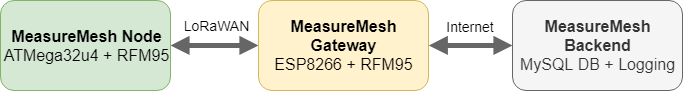
\includegraphics[width=8cm]{images/ComonentOverview.png}
    \caption{Communication model showing system components and their hardware implementation.}
    \label{fig:mmoverview}
\end{figure}


There are five major components of MeasureMesh, they can be seen listed in Table \ref{tab:schedule}, along with their completion status. MeasureMesh nodes consist of an Adafruit Radiofruit ATMega32u4 (Arduino programmable), with an on-board RFM95 LoRa compliant radio module \footnote{https://www.adafruit.com/product/3078}. This Radiofruit also includes a LiPo battery charger and USB connection for programming. In order to house these components, a 3D-printable enclosure was designed in CAD. The 3D printed version of this enclosure, with the Node hardware inside, can be seen in Fig. \ref{fig:nodeproto}. 


\begin{figure}
    \centering
    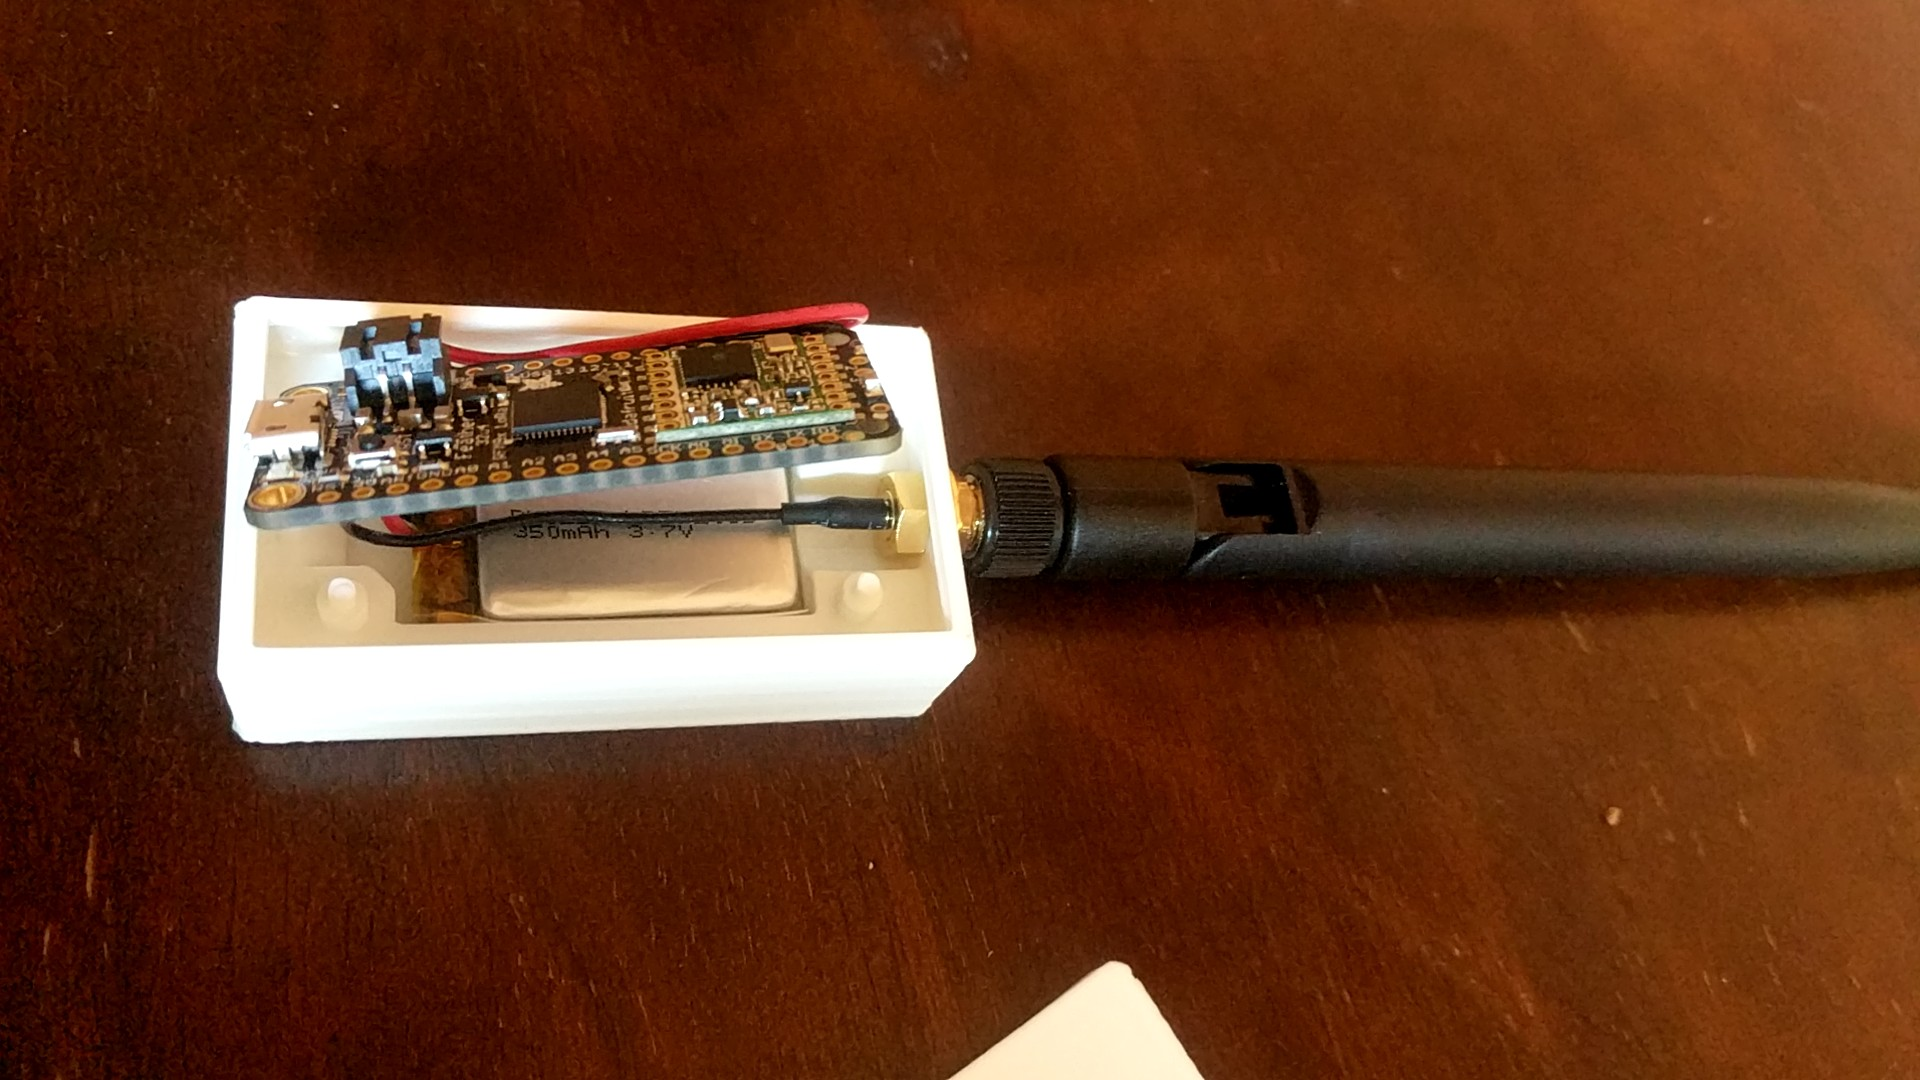
\includegraphics[width=8cm]{images/nodePrototype}
    \caption{MeasureMesh Node prototype, with enclosure, battery and antenna.}
    \label{fig:nodeproto}
\end{figure}

The same LoRa radio module is also available a a breakout board without the 32u4 processor\footnote{https://www.adafruit.com/product/3072}. This board is used in combination with a commodity ESP8266 development board to create the LoRa $\Longleftrightarrow$ WiFi gateway node. This assembled hardware is functional and has passed basic operations testing. It is shown in Fig. \ref{fig:gatewayproto}.

\begin{figure}
    \centering
    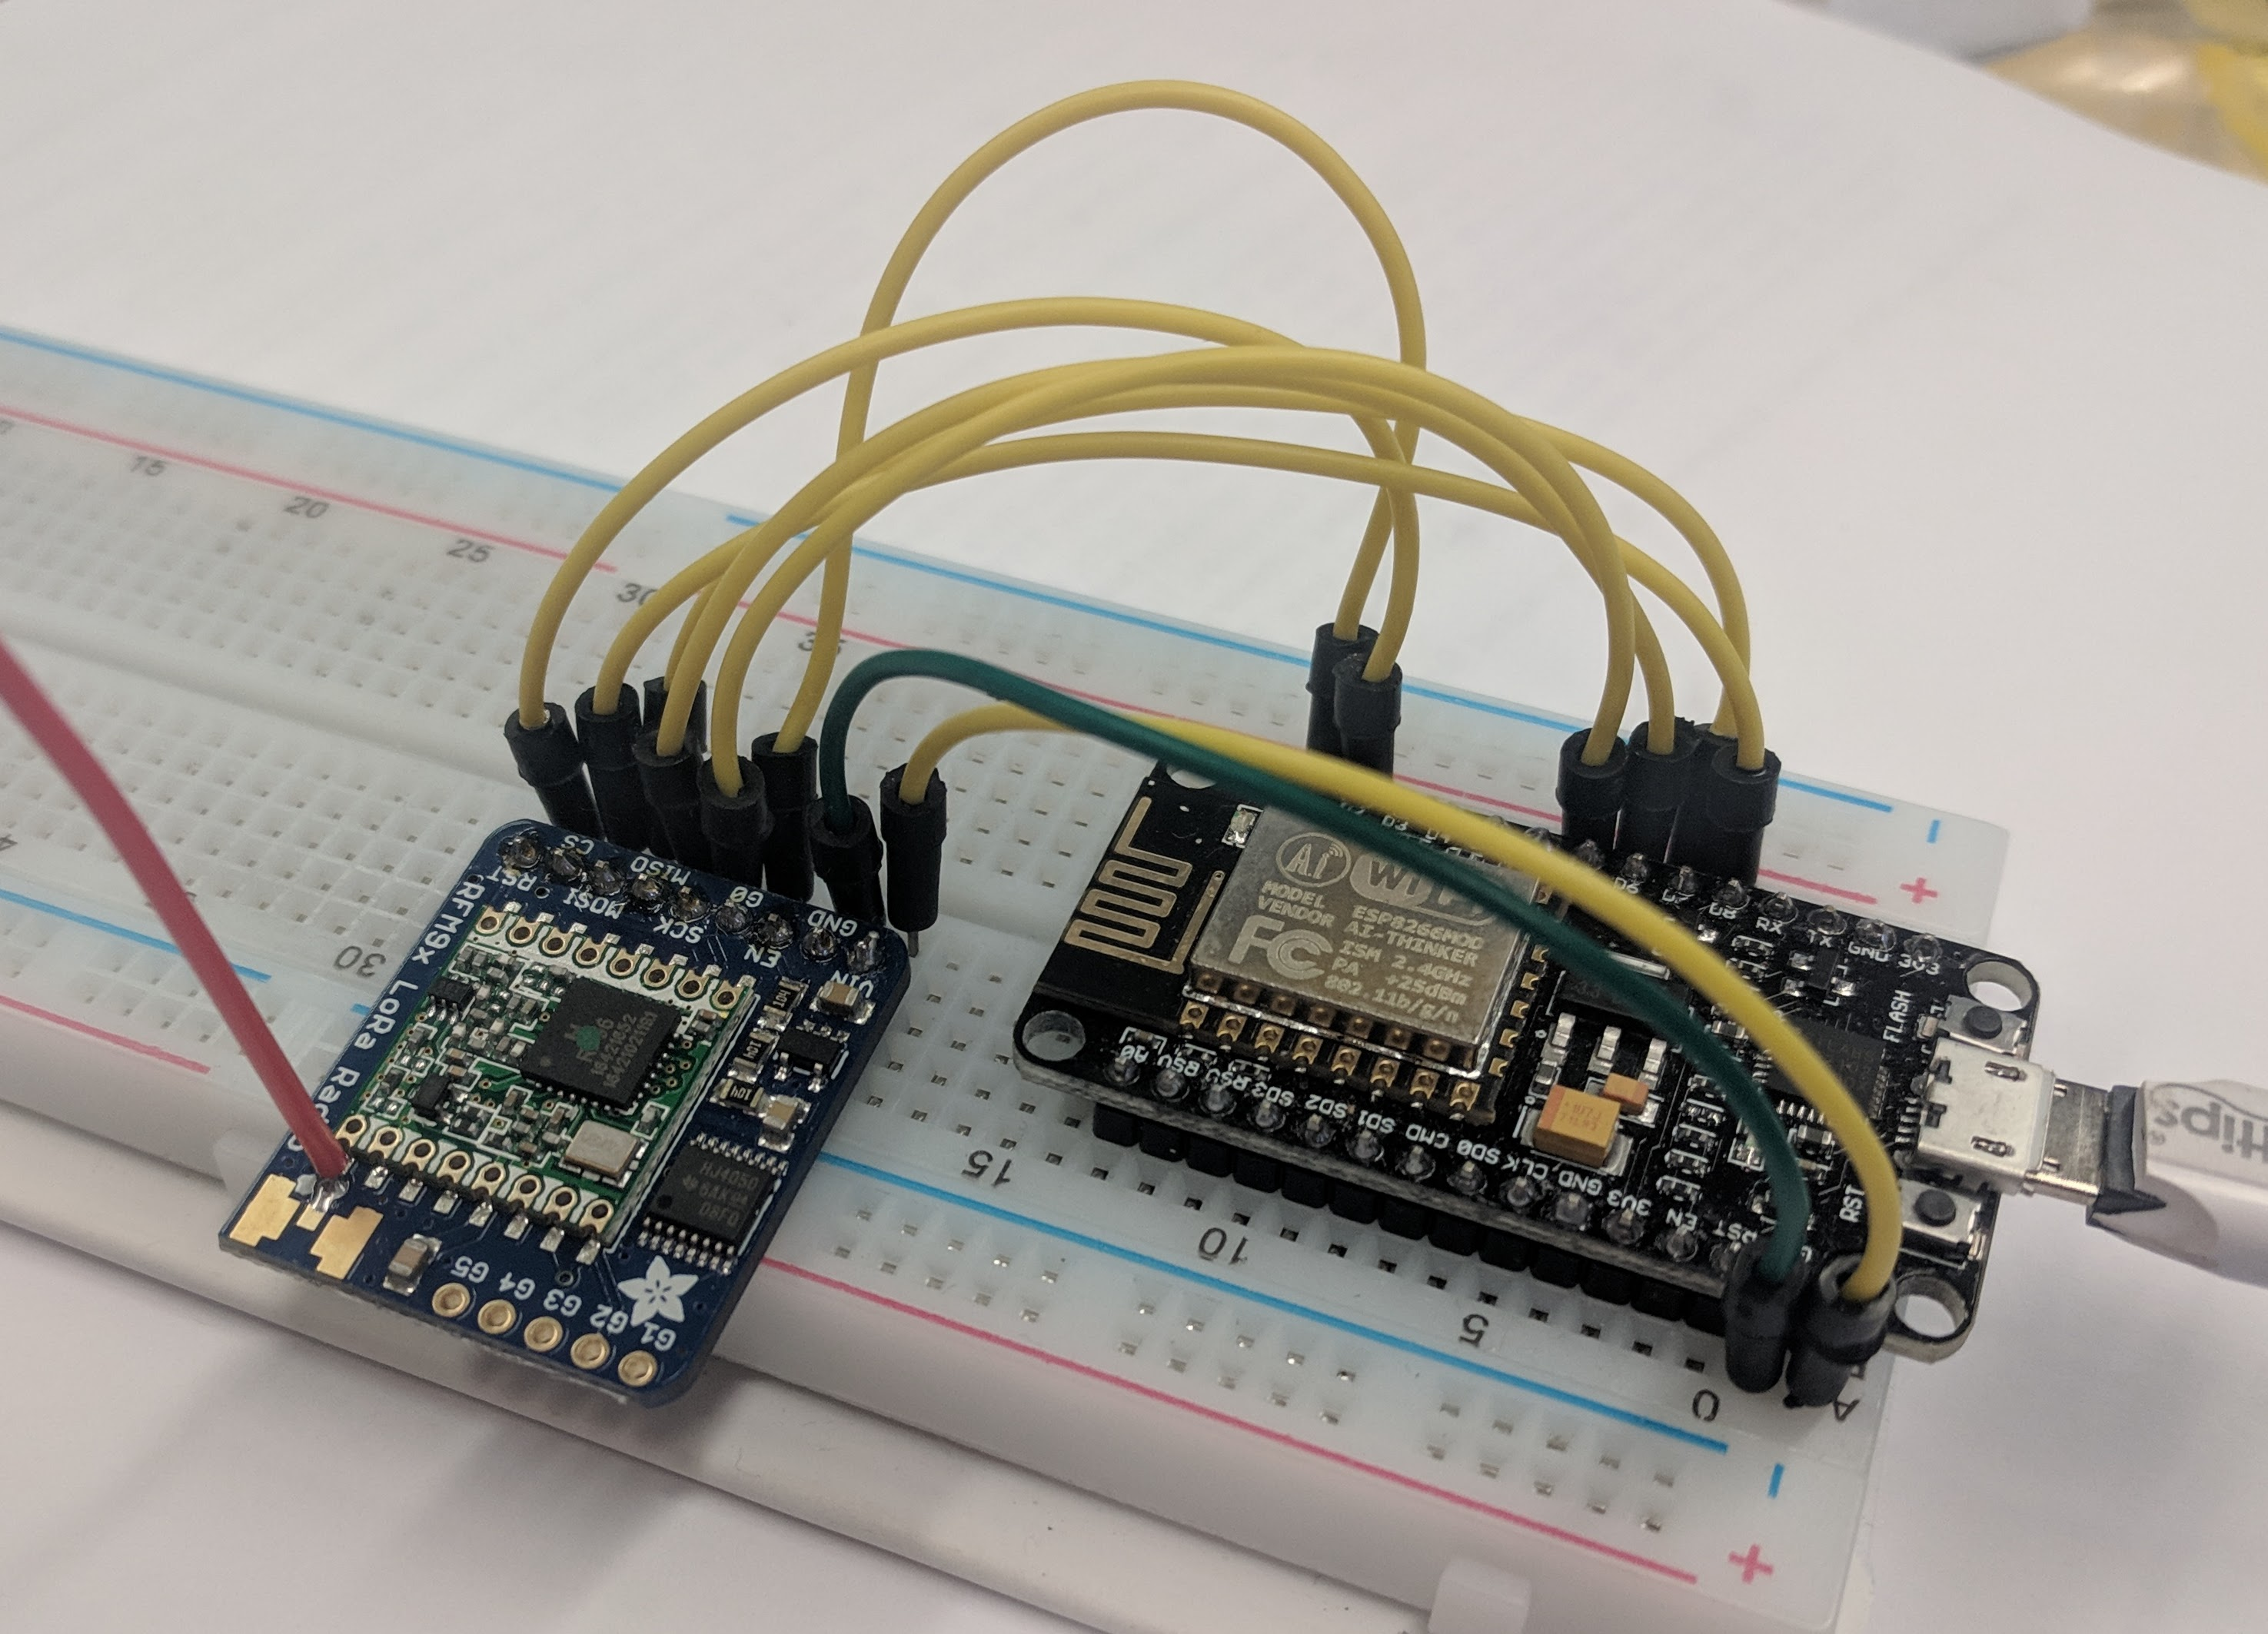
\includegraphics[width=8cm]{images/gatewayPrototype.jpg}
    \caption{MeasureMesh Gateway hardware prototype, without enclosure.}
    \label{fig:gatewayproto}
\end{figure}

A MeasureMesh node reports its chosen sensor data along with certain meta information such as battery life, Node ID, and the context of the reading it is transmitting (temperature, humidity, light level, etc). MeaureMesh nodes are highly configurable in software and support varying logging intervals, sleeping in between transmitting for maximum power savings as well as multiple sensors per node. 

A MeasureMesh Gateway device acts as a bridge between the LoRa radio and the MeasureMesh back-end. The Gateway is always listening for LoRa packets. When one is received, it interprets the information and forms an HTTP (REST) request to be sent to the MeasureMesh database over the internet. This database address is configurable and may be a local computer or a live website.

The data is stored according to Node and Gateway ID. The user can then browse  a list of available 'streams' of information that have been logged from the Nodes through the Gateway. A user can select one or more of these streams and plot them over an arbitrary timescale. The units of the plots will be according to the metadata associated with each node. 

\begin{figure}
    \centering
    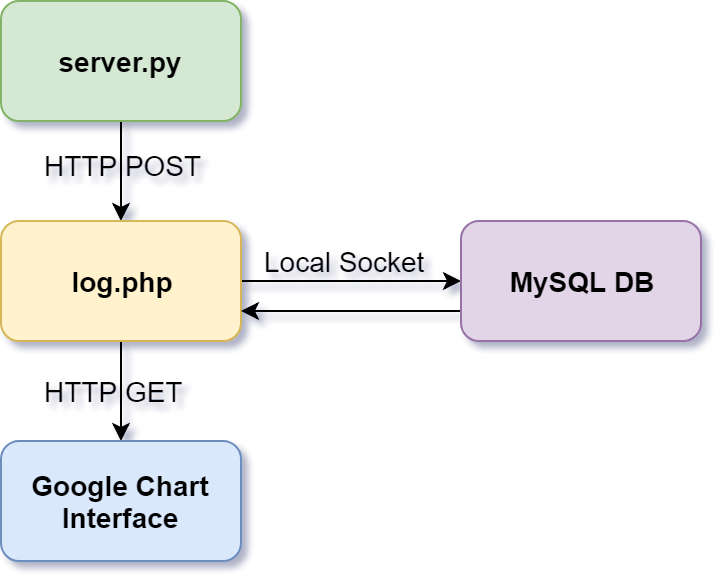
\includegraphics[width=6cm]{images/mm-user-interface}
    \caption{MeasureMesh Server diagram.}
    \label{fig:mm-ui-data}
\end{figure}


%%%%%%%%%%%%%%%%%%%%%%%%%%%%%
%%%%%%%%%%%%%%%%%%%%%%%%%%%%%
%%%%%%%%%%%%%%%%%%%%%%%%%%%%%
%%%%%%%%%%%%%%%%%%%%%%%%%%%%%
\section{Learning Outcome}

This project is providing an opportunity to explore state of the art radio communication standards that are currently being deployed on a commercial IoT scale. The improved range and lower power consumption that is offered by LoRa radios allows for an even sparser grid of sensors that can last even longer on a given battery, or more efficiently utilize solar power. 

It is also interesting to experiment with actual resulting range differences between urban and rural environments, and line-of-sight versus obstructed communication paths. This will definitely come in to play when recommending Node placements to the end users of MeasureMesh.


\bibliographystyle{ieeetr}
\bibliography{refs.bib}

\end{document}
